\begin{frame}{Permutation pattern}
    \begin{block}{Definition}<1->
    A permutation $\pi$ \emph{contains} another permutation $\sigma$ if a subsequence of $\pi$ has the same relative order as $\sigma$, denoted $\contains{\pi}{\sigma}$.
    \end{block}
    \begin{block}{Definition}<1->
    A permutation $\pi$ \emph{avoids} $\sigma$ if it does not contain it.
    \end{block}
    \only<2>{%
    \begin{figure}
        \centering
        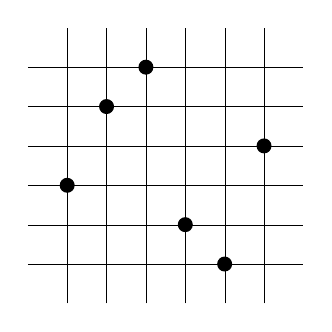
\begin{tikzpicture}[scale=.5,baseline=(current bounding box.center)]
\foreach \x in {1,...,6} {
    \draw[ultra thin] (\x,0)--(\x,7); %vline
    \draw[ultra thin] (0,\x)--(7,\x); %hline
}
\draw[fill=black] (1,3) circle (5pt);
\draw[fill=black] (2,5) circle (5pt);
\draw[fill=black] (3,6) circle (5pt);
\draw[fill=black] (4,2) circle (5pt);
\draw[fill=black] (5,1) circle (5pt);
\draw[fill=black] (6,4) circle (5pt);
\end{tikzpicture}
        \caption{The permutation $356214$.}
    \end{figure}
    }
    \addtocounter{figure}{1}
    \onslide<3->{%
    \begin{figure}
        \centering
        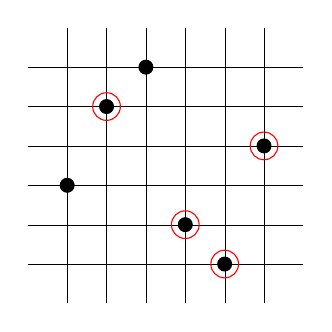
\begin{tikzpicture}[scale=.5,baseline=(current bounding box.center)]
\foreach \x in {1,...,6} {
    \draw[ultra thin] (\x,0)--(\x,7); %vline
    \draw[ultra thin] (0,\x)--(7,\x); %hline
}
\draw[fill=black] (1,3) circle (5pt);
\draw[fill=black] (2,5) circle (5pt);
\draw[fill=black] (3,6) circle (5pt);
\draw[fill=black] (4,2) circle (5pt);
\draw[fill=black] (5,1) circle (5pt);
\draw[fill=black] (6,4) circle (5pt);
\draw<3->[red] (2,5) circle (10pt);
\draw<3->[red] (4,2) circle (10pt);
\draw<3->[red] (5,1) circle (10pt);
\draw<3->[red] (6,4) circle (10pt);
\end{tikzpicture}
        \caption{An occurrence of $4213$ in $356214$.}
    \end{figure}
    }
\end{frame}